\section{Introduction}

\cite{fabre_shortfall_2025} assesses whether growth and domestic redistribution can eradicate extreme poverty by 2030, the first target of the Sustainable Development Goals. It relies on PIP data downloaded in 2023, expressed in 2017 PPP~\$, with the extreme poverty line at \$2.15/day. The paper noted that its estimates ``could be improved when PIP releases a data update''. Since then, the World Bank has adopted the 2021 PPPs together with revised poverty lines \citep{foster_global_2025}, and has incorporated many new surveys, most recently in its September 2026 update \citep{castaneda_aguilar_september_2026}. With four years remaining before 2030, this note re-runs the original code on the latest data.

\section{Method}

The method is unchanged from \cite{fabre_shortfall_2025}. For each country, PIP provides the percentiles of the per capita consumption (or income) distribution in the most recent survey year. I project each percentile to 2022 using the observed growth of GDP per capita between the survey year and 2022, and then to 2030 under various growth scenarios, assuming balanced growth (i.e. constant national inequality). For surveys conducted after 2022, observed growth between 2022 and the survey year is used to bring the distribution back to 2022. In other words, the growth scenarios always apply to the period 2022--2030 and observed growth is used for all years between the survey and 2022. Additionally, I introduce a scenario that uses observed growth up to the last year with data (2025 for most countries) followed by 3\% annual growth. For the few countries lacking GDP data, the scenario growth rate is applied from the survey year onwards, as in the original paper. I then compute, for each country in 2030, the \textit{antipoverty cap} (the threshold above which all income would need to be confiscated to close the poverty gap), the \textit{antipoverty tax} (the linear tax rate above a given threshold needed to close the poverty gap) and the \textit{income floor} that a given tax could finance. These idealized policies abstract from administrative costs and behavioral responses: they provide upper bounds of domestic capacity.

\section{What changed}

\paragraph{Poverty lines.} The international poverty lines become \$3.00 (formerly \$2.15), \$4.20 (formerly \$3.65), and \$8.30 (formerly \$6.85) per person per day, in 2021 PPP~\$. These new lines are not mere price conversions of the former ones. Converted to 2021 prices, the \$2.15 line would be worth \$2.46; most of the rise to \$3.00 reflects higher national poverty lines in low-income countries, themselves due to surveys that capture more consumption \citep{foster_global_2025}. The \$3.00 line is thus a higher bar in real terms. To separate the effect of the new data from that of the higher line, I present results both at the new lines and at the price-equivalent lines of \$2.46 and \$7.84 (i.e. \$6.85 scaled by the same factor of 2.46/2.15). The taxation threshold of the antipoverty tax and income floor is set at the acute poverty line in each case (\$8.30 or \$7.84). The threshold of \$18.15/day, which corresponds to the 2021 U.S. federal poverty line for a family of four (\$26,500 a year), is already expressed in 2021~\$ and is kept unchanged, as is the threshold of \$100/day for the global tax.

\paragraph{Surveys.} The PIP data (version 20260922) cover 172 economies, of which \upNbCountries{} are included in the analysis (vs. 167 in the original paper; as before, Taiwan is excluded for lack of GDP data). Among the 168 countries covered by both vintages, the most recent survey has changed for 118. \upShareSurveyRecent\% of countries now have a survey from 2021 or later (vs. 59\% surveyed between 2018 and 2021 in the original data). The update is particularly consequential for the poorest countries. The most recent survey dates from 2020 instead of 2012 for the D.R.\ Congo, from 2021 instead of 2012 for Madagascar, 2020 instead of 2013 for Burundi, 2021 instead of 2015 for Ethiopia, 2021 instead of 2008 for the Central African Republic, 2022 instead of 2014 for Mozambique, and 2022 instead of 2018 for Nigeria. For India, the 2023--24 Household Consumption Expenditure Survey replaces the 2019 data. It shows a sharp fall in extreme poverty, which the World Bank recommends interpreting with caution, as it may partly reflect improvements in survey implementation \citep{castaneda_aguilar_september_2026}.

\paragraph{Growth.} GDP per capita (in constant 2021 PPP~\$) now comes from the World Development Indicators of October 2026, which run through 2025. Surveys conducted after 2022 are therefore brought back to 2022 using observed growth. To keep results comparable, the growth scenarios are still defined over 2022--2030. I add one scenario that uses observed growth over 2022--2025, followed by a 3\% annual growth up to 2030. Household final consumption (used in the robustness check that rescales survey data to national accounts) is updated from the same source.

\paragraph{Code.} Two minor issues are fixed. First, as PIP now provides a national distribution for China, it is used directly rather than reconstructed from the urban and rural distributions (the original data did not include a national distribution, so the original results are unaffected). Second, the list of low-income countries contained two coding errors, which are corrected (Sierra Leone was miscoded and the Central African Republic was missing).\footnote{This only affects the statistics on low-income countries, which now number 28. In the original paper, the correction would leave the average antipoverty tax in low-income countries unchanged (70\%), and raise from 13 to 14 the number of low-income countries unable to finance an income floor at \$2.15/day with a 10\% tax above \$6.85/day.} The code and data are available at \href{https://github.com/bixiou/domestic_poverty_eradication}{github.com/bixiou/domestic\_poverty\_eradication} (see \texttt{code\_poverty/update.R}).

\section{Updated results}

\begin{table}[h]

\caption[Global poverty (rates and gaps) in 2030 under different growth scenarios (September 2026 PIP data).]{\label{tab:poverty_update}Global poverty rates and poverty gaps in 2030 under different growth scenarios, using the September 2026 PIP data. Poverty rates are expressed in \% of world population and poverty gaps in \% of world GDP. Poverty lines are in 2021 PPP \$/day.}
\centering
\begin{tabular}[t]{lrrrrrrrr}
\toprule Growth scenario & \multicolumn{4}{c}{Poverty rate (\%)} & \multicolumn{4}{c}{Poverty gap (\% of GDP)} \\ 
 (Poverty line in \$/day)  & 3.00 & 4.20 & 8.30 & 18.15 & 3.00 & 4.20 & 8.30 & 18.15\\
\midrule
2022 Estimate & 10.0 & 19.0 & 47.9 & 71.6 & 0.49 & 1.32 & 8.36 & 38.30\\
Trend (2014--2019) & 8.5 & 13.8 & 36.2 & 65.4 & 0.39 & 0.94 & 5.03 & 26.63\\
Max(Trend, 0) & 8.0 & 13.2 & 35.8 & 65.2 & 0.36 & 0.88 & 4.87 & 26.25\\
Autoregressive projection & 7.9 & 14.0 & 39.5 & 65.9 & 0.33 & 0.87 & 5.43 & 28.00\\
3\% growth & 7.1 & 13.2 & 40.0 & 67.2 & 0.28 & 0.76 & 5.15 & 27.34\\
3\% unbalanced growth & 6.8 & 12.1 & 38.0 & 66.6 & Inf & Inf & Inf & Inf\\
7\% growth & 3.8 & 7.4 & 25.9 & 58.1 & 0.11 & 0.30 & 2.22 & 15.23\\
7\% growth since 2016 & 1.6 & 3.5 & 15.5 & 49.1 & 0.03 & 0.09 & 0.85 & 8.06\\
Observed to 2025, then 3\% & 7.6 & 13.3 & 38.5 & 66.6 & 0.31 & 0.81 & 5.08 & 27.21\\
\bottomrule
\end{tabular}
\end{table}

\paragraph{Growth alone.} Table \ref{tab:poverty_update} updates Table 1 of \cite{fabre_shortfall_2025} at the new poverty lines. I estimate that \upRatePovNow\% of the world population lived below \$3.00/day in 2022, somewhat below the World Bank's official estimate of 10.9\%, a gap similar to that in the original paper.\footnote{The difference partly comes from countries without PIP data, which are excluded here while the World Bank imputes their poverty, and from differences in the way survey data are extrapolated to 2022 using national accounts.} With a balanced growth of 3\% per year, extreme poverty would still affect \upRatePovThree\% of the world population in 2030 (\upRatePovThreeEq\% at the price-equivalent line of \$2.46, vs. 5.2\% in the original paper). Accounting for the observed growth over 2022--2025, which fell short of 3\% per capita per year in 15 of the 22 low-income countries with data, raises this figure to \upRatePovRealized\% (\upRatePovRealizedEq\% at \$2.46). Even with 7\% annual growth, extreme poverty would remain at \upRatePovSeven\% (\upRatePovSevenEq\% at \$2.46, exactly as in the original paper), and at \upRatePovSDG\% had this growth started in 2016. The extreme poverty gap amounts to \upGapThree\% of world GDP in 2030 in the 3\% growth scenario (\upGapThreeEq\% at \$2.46, vs. 0.14\%).

\paragraph{Domestic redistribution.} Table \ref{tab:comparison} compares the main results with the original ones, and Figure \ref{fig:tax} shows the antipoverty tax in the countries where it is highest. At the price-equivalent lines, domestic capacity is very close to the original estimates. In the 3\% growth scenario, taxing all income above \$7.84/day at 100\% would not suffice to eradicate extreme poverty in \upNbCapEq{} countries (vs. 5): \upCountriesCapEq. The average antipoverty tax in Sub-Saharan Africa is unchanged at \upTaxEqSSA\%, and a 10\% tax above \$7.84/day would not finance an income floor at \$2.46/day in \upNbFloorEq{} countries (vs. 23). At the new, higher lines, the shortfall is more severe. Taxing all income above \$8.30/day would not suffice in \upNbCapEight{} countries, all of them low-income: \upCountriesCapEight. In the D.R.\ Congo, mean consumption would remain below \$3.00/day in 2030, so that even a full equalization of incomes would not end extreme poverty. Madagascar, which was in this situation with its 2012 survey, no longer is with its 2021 survey (mean consumption reaches \$\upMeanThreeMDG/day in 2030). On average, the antipoverty tax above \$8.30/day would be \upTaxEightSSA\% in Sub-Saharan Africa and \upTaxEightLIC\% in low-income countries. A 10\% tax above \$8.30/day would not finance an income floor at \$3.00/day in \upNbFloor{} countries, including \upNbFloorLIC{} of the 28 low-income countries. Even if a 7\% growth had started in 2016, this tax would not suffice in \upNbFloorSDG{} countries: \upCountriesFloorSDG.

\begin{figure}[h]
\caption{\label{fig:tax}Tax rate on consumption above a threshold needed to eradicate extreme poverty in 2030, assuming 3\% annual growth (countries with a rate of at least 40\% at the new line; bars truncated at 250\%).}
\centering
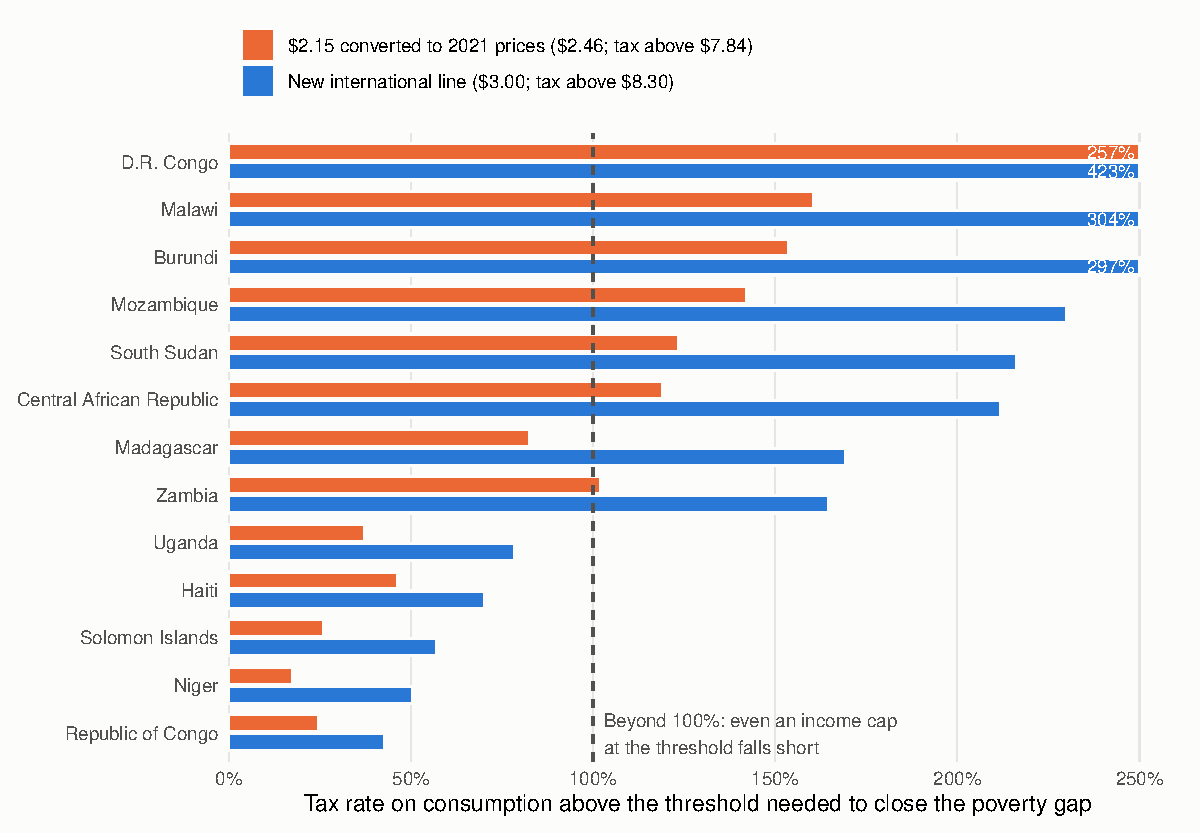
\includegraphics[width=\textwidth]{../figures/tax_by_country.pdf}
\end{figure}

India stands out. With the new surveys, extreme poverty in India would be down to \upRateThreeIND\% in 2030 in the 3\% growth scenario, and the antipoverty tax above \$18.15/day would be just \upTaxEighteenThreeIND\% (vs. 156\% previously). India now clearly appears able to eliminate extreme poverty with its domestic resources, subject to the caveats on its latest survey.

\paragraph{Global redistribution.} Closing the global extreme poverty gap at \$3.00/day in 2030 would require a \upRateHundred\% marginal tax on income above \$100/day (\upRateHundredEq\% at \$2.46, vs. 1.2\% originally), or \upRateHundredHFCE\% when survey data are rescaled to national accounts. \upShareBelowHundred\% of the world population lives below this threshold. A global 10\% tax above \$8.30/day would finance a global income floor of \$\upGlobalFloor/day and reduce the global Gini from \upGiniThree{} to \upGiniThreeGlobalTax.

\begin{table}[h]
\caption{\label{tab:comparison}Main results: original paper vs. update.}
\centering
\makebox[\textwidth][c]{
\begin{tabular}{lccc}
\toprule
 & \makecell{Fabre (2025)\\ 2017 PPP} & \makecell{Update, 2021 PPP\\ equivalent lines} & \makecell{Update, 2021 PPP\\ new lines} \\
\midrule
Extreme poverty line (\$/day) & 2.15 & 2.46 & 3.00 \\
Acute poverty line / taxation threshold (\$/day) & 6.85 & 7.84 & 8.30 \\
\midrule
\textit{Extreme poverty rate (\% of world population)} & & & \\
\quad 2022 estimate & 7.3 & \upRatePovNowEq & \upRatePovNow \\
\quad 2030, 3\% growth & 5.2 & \upRatePovThreeEq & \upRatePovThree \\
\quad 2030, 7\% growth & 2.2 & \upRatePovSevenEq & \upRatePovSeven \\
\quad 2030, 7\% growth since 2016 & 1.1 & \upRatePovSDGEq & \upRatePovSDG \\
Extreme poverty gap in 2030, 3\% growth (\% of world GDP) & 0.14 & \upGapThreeEq & \upGapThree \\
\midrule
\textit{Domestic capacity in 2030, 3\% growth} & & & \\
\quad Countries where a cap at the acute line is insufficient & 5 & \upNbCapEq & \upNbCapEight \\
\quad Antipoverty tax above the acute line: Sub-Saharan Africa (\%) & 46 & \upTaxEqSSA & \upTaxEightSSA \\
\quad Antipoverty tax above the acute line: Nigeria (\%) & 20 & \upTaxEqNGA & \upTaxEightNGA \\
\quad Antipoverty tax above \$18.15/day: India (\%) & 156 & \upTaxEighteenThreeINDEq & \upTaxEighteenThreeIND \\
\quad Countries where a 10\% tax above the acute line & & & \\
\quad \quad cannot finance an income floor at the extreme line & 23 & \upNbFloorEq & \upNbFloor \\
\quad \quad idem, with 7\% growth & 10 & \upNbFloorSevenEq & \upNbFloorSeven \\
\quad \quad idem, with 7\% growth since 2016 & 1 & \upNbFloorSDGEq & \upNbFloorSDG \\
\midrule
\textit{Global redistribution in 2030, 3\% growth} & & & \\
\quad Tax rate above \$100/day closing the extreme poverty gap (\%) & 1.2 & \upRateHundredEq & \upRateHundred \\
\quad Income floor from a 10\% tax above the acute line (\$/day) & 8.6 & \upGlobalFloorEq & \upGlobalFloor \\
\bottomrule
\end{tabular}}
\end{table}

\section{Conclusion}

The new data confirm the main conclusion of \cite{fabre_shortfall_2025}: neither growth alone nor growth combined with radical domestic redistribution can eradicate extreme poverty by 2030. At price-equivalent poverty lines, the results are remarkably stable despite the renewal of most surveys. At the new international poverty line, which sets a higher bar, the shortfall of domestic resources is more severe and concentrated in low-income countries of Sub-Saharan Africa, while India no longer appears to be a borderline case. Although the cost of eradicating extreme poverty at \$3.00/day represents about twice as large a share of global income as at \$2.15/day, it remains modest, at \upGapThree\% of global income. This illustrates the potential of international solidarity.
